\documentclass[12pt,a4paper]{article}
\usepackage[margin=2cm]{geometry}
\usepackage{xeCJK}
\usepackage{fontspec}
\setCJKmainfont{Noto Serif CJK TC}[Script=CJK]
\setCJKmonofont{Noto Sans Mono CJK TC}[Script=CJK]
\usepackage{amsmath,amssymb}
\usepackage{graphicx}
\usepackage{fancyhdr}
\setlength{\headheight}{14.5pt}
\addtolength{\topmargin}{-2.5pt}
\usepackage{hyperref}
\usepackage{xcolor}
\usepackage{listings}
\usepackage{enumitem}
\usepackage{titlesec}
\usepackage{caption}
\usepackage{indentfirst}
\usepackage{tikz}
\setlength{\parindent}{2em}
\pagestyle{fancy}
\fancyhf{}
\cfoot{\thepage}
\linespread{1.3}
\fancyhead[L]{\nouppercase{\leftmark}}

\lstset{
    basicstyle=\ttfamily\footnotesize,  % 字型與大小
    keywordstyle=\color{blue},
    commentstyle=\color{gray},
    stringstyle=\color{orange},
    numbers=left,                       % 行號在左側
    numberstyle=\tiny\color{gray},
    stepnumber=1,                       % 每行都顯示行號
    numbersep=5pt,
    backgroundcolor=\color{white},
    frame=single,                       % 加上框線
    breaklines=true,                    % 長行自動換行
    tabsize=2,
    language=C++                     % 可以換成 \texttt{C++}, \texttt{Java}, etc.
}

\title{\texttt{Arduino}教學手冊}
\author{Tai, Wei-Hsuan}
\date{\today}

\begin{document}

\maketitle

\lhead{\texttt{Arduino}教學手冊}
\rhead{2025/07/05}
\newpage
\tableofcontents
\newpage

\newpage
\section{\texttt{Arduino}介紹}

平時你在寫程式時,會使用電腦的中央處理器(\texttt{CPU})來執行程式碼,
而\texttt{Arduino}的核心就是一顆微處理器,這顆微處理器可以執行你寫的程式碼,
並且控制外部的電子元件,例如\texttt{LED}燈、馬達、感測器等等。

\texttt{Arduino}的開發環境是\texttt{Arduino IDE},這是一個可以讓你寫程式、編譯程式、上傳程式到\texttt{Arduino}開發板的軟體,
我們已經幫你們安裝好了,但如果你在家裡想要嘗試,可以去\texttt{https://www.arduino.cc/en/software}下載最新版本的\texttt{Arduino IDE}。

\section{電子學的基本概念}

\subsection{電壓(\texttt{Voltage})}
電壓是電流的驅動力,單位是伏特(\texttt{Volt}),簡稱\texttt{V}。電阻相同時,電壓越高,電流越大。

\subsection{電流(\texttt{Current})}
電流是電荷的流動,單位是安培(\texttt{A}),簡稱\texttt{I}。電流越大,代表單位時間內通過的電荷量越多。

\subsection{電阻(\texttt{Resistance})}
電阻是對電流流動的阻礙,單位是歐姆($\Omega$),簡稱\texttt{R}。在相同電壓下電阻越大,電流越小。

\subsection{歐姆定律(\texttt{Ohm's Law})}
電壓、電流和電阻之間關係,可以使用歐姆定律來表示,公式為:
$$
V = I \cdot R
$$

這個公式告訴我們,當電壓不變時,電流和電阻成反比;當電阻不變時,電流和電壓成正比。

如果用水管來比喻,電壓就是水壓,電流就是水流的速度,電阻就是水管的阻塞程度,
水壓越大,水流的速度越快;水管阻塞程度越大,水壓就越大。

\section{如何透過\texttt{Arduino}控制元件}

當 \texttt{Arduino} 的腳位輸出電壓,並透過電路接到元件(例如 LED 或馬達)時,元件會因為電壓差而產生電流。這個電流流經元件內部,讓它發光、發聲或轉動。
這就是 \texttt{Arduino} 控制元件的基本原理。這一部份的內容會教你如何使用程式控制 \texttt{Arduino} 的腳位輸出電壓,並透過電路接到元件。

\subsection{元件介紹}
在這一部份,我們將介紹一些常用的電子元件,這些元件可以用來控制電路的狀態,並且可以與Arduino開發板進行互動。

\subsubsection{LED}

LED是發光二極體(light-emitting diode)的縮寫,簡言之是個通電之後會發光的元件。
觀察LED燈泡,你會發現有一長一短的兩隻腳,在連接電路時,長腳是正極,短腳是負極。

LED非常容易燒壞,所以在連接電路時,必須加上電阻來保護LED。
電阻的計算尤其複雜,這邊不贅述,直接使用我們給你的就行了

\subsubsection{電阻}
電阻是用來限制電流流動的元件,在電路中通常與電子元件串聯使用,以防止電流過大導致電子元件損壞。
串聯電阻可以「分擔部分電壓」,藉此控制通過元件的電流大小。選擇合適的電阻值非常重要,這取決於電源電壓、
元件的順向電壓與其額定電流。


\subsubsection{麵包板}

麵包板是電子電路設計常用的基底,上面佈滿孔洞,孔洞底下藏有金屬導軌,可直接插入電子元件而不需焊接,方便修改與重組。

將麵包板橫放時,
最上方與最下方各有兩條電源軌,同一條電源軌在水平方向導通;
中間端子區以中心缺口為界分成左右兩半。每半邊「同一列連續 5 個孔」垂直導通,相鄰列與另一半邊互不相通。
下圖示意了上述連通方式(紅/藍橫線為電源軌,灰色虛線為中心缺口)。

\begin{center}
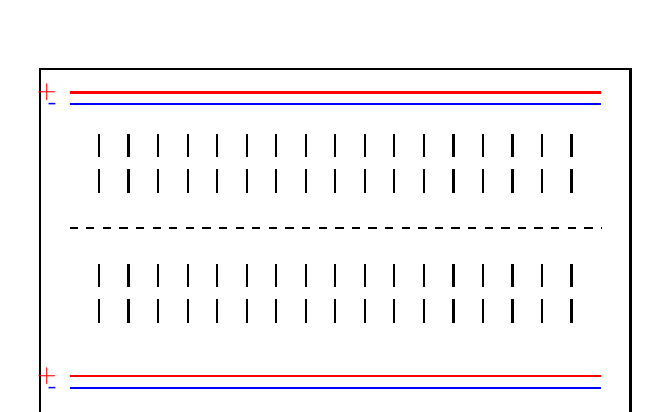
\begin{tikzpicture}[font=\small, scale=0.75]

%---------------- 尺寸參數 ----------------%
\def\leftX{0}     % 外框左
\def\rightX{10}   % 外框右
\def\topY{6}      % 外框上
\def\botY{0}      % 外框下
\def\gapY{3.3}    % 中心 Gap (虛線) 的 y 座標
\def\railDy{0.2}  % Power rail 兩條線的間距
\def\holeLen{0.4} % 每支垂直線長度
\def\rowSep{0.6}  % 垂直洞列與中心 gap 的距離

%---------------- 外框 ----------------%
\draw[thick] (\leftX,\botY) rectangle (\rightX,\topY);

%---------------- Power rails ----------------%
\foreach \y/\col in {5.6/red, 5.4/blue, 0.8/red, 0.6/blue} {
\draw[\col, thick] (0.5,\y) -- (9.5,\y);
}
% + / - 標示
\node[anchor=east, red ] at (0.45,5.6) {+};
\node[anchor=east, blue] at (0.45,5.4) {-};
\node[anchor=east, red ] at (0.45,0.8) {+};
\node[anchor=east, blue] at (0.45,0.6) {-};

%---------------- Terminal strips ----------------%
\foreach \x in {1,1.5,...,9} {%
% 上半兩列(離中心 gap 同距離 rowSep)
\draw[thick] (\x,\gapY+\rowSep+\holeLen) -- (\x,\gapY+\rowSep);
\draw[thick] (\x,\gapY+2*\rowSep+\holeLen) -- (\x,\gapY+2*\rowSep);
% 下半兩列(對稱)
\draw[thick] (\x,\gapY-\rowSep) -- (\x,\gapY-\rowSep-\holeLen);
\draw[thick] (\x,\gapY-2*\rowSep) -- (\x,\gapY-2*\rowSep-\holeLen);
}

%---------------- 中心 Gap (一次畫到底) ----------------%
\draw[dashed, thick] (0.5,\gapY) -- (9.5,\gapY);

\end{tikzpicture}
\end{center}

\subsubsection{蜂鳴器}
蜂鳴器是個很吵的元件,當你給它一個電壓訊號時,它會發出聲音,
你可以利用電壓的大小來控制音量的大小,利用電壓的頻率來控制音調的高低。

蜂鳴器的使用方式與LED一樣,只要將蜂鳴器的正極連接到開發板的腳位,負極連接到GND腳位,
然後使用\texttt{digitalWrite()}來控制腳位的電壓輸出,就可以讓蜂鳴器發出聲音。和LED不同的地方是,
蜂鳴器也有內電阻,所以不需要額外加上電阻來保護它。


\subsubsection{壓覺感測器}

檢查你手中的元件盒,你會發現似乎沒有按鈕這個元件,這是因為我們使用了壓覺感測器來取代按鈕。
壓覺感測器就是個觸控開關,當你觸碰它時,會產生一個電壓訊號,這個電壓訊號可以用來控制其他元件的狀態。

電路的部份,他需要一組單獨的電源來供電,這組電源的正極連接到壓覺感測器的VCC腳位,負極連接到GND腳位,
而壓覺感測器的SIG腳位則連接到開發板的腳位,
這樣就可以使用\texttt{digitalRead()}來讀取壓覺感測器的電壓訊號。
壓覺感測器有內電阻,所以不需要額外加上電阻來保護它。

\subsubsection{Arduino Uno開發板}
就是你手上這一塊開發板,這是Arduino的入門款開發板,連接電腦後可以透過程式控制每個腳位的行為,
這裡不贅述(因為可以講的太多了)。



\subsection{Arduino IDE的程式結構}
Arduino IDE的程式結構主要由三個部分組成:設定區、主程式區和函式區。設定區用於初始化變數和設定腳位,主程式區則是執行的主要邏輯,而函式區則是用來定義可重複使用的函式。

以下的程式碼是你一打開Arduino IDE就會看到的範本程式碼:
\begin{lstlisting}
void setup() {
  // put your setup code here, to run once:
}
void loop() {
  // put your main code here, to run repeatedly:
}
\end{lstlisting}

其中,\texttt{setup()}函式是用來初始化變數和設定腳位的,這個函式只有在每次重新啟動時會執行一次,
而\texttt{loop()}函式則是用來執行主要邏輯的,這個函式會不斷重複執行,直到電源關閉或\texttt{Arduino}被重置。

一般而言,我們會在\texttt{setup()}函式中設定腳位的模式,例如輸入或輸出,然後在\texttt{loop()}函式中執行主要邏輯,例如讀取感測器的數據或控制元件的狀態。

你可以觀察到Arduino IDE的程式碼結構一樣是使用無數個函式來組成的,因此全域變數、自訂函式、類別等概念在Arduino IDE中也一樣適用,
但請記得考量到Arduino開法板的效能,盡量避免使用過多的全域變數與類別,這樣會影響程式的執行速度。

\subsection{\texttt{Arduino}的輸出}
平時使用電腦編譯\texttt{C++}程式時,會使用\texttt{cout}來輸出結果,
但在使用\texttt{Arduino}時,執行程式的核心不是電腦的\texttt{CPU},而是你手上那一塊\texttt{Arduino}開發板,
所以我們不能使用\texttt{cout}來輸出結果,因為\texttt{Arduino}開發板並沒有螢幕可以顯示結果。
而是使用\texttt{Serial}來輸出結果,這樣\texttt{Arduino}開發板就可以透過USB線將結果傳送到電腦上,
然後電腦就可以使用\texttt{Serial Monitor}來顯示結果。

這樣的作法等同於僅借用電腦的螢幕來顯示結果,電腦本身不參與運算。

\begin{lstlisting}
Serial.println("Hello World!"); //輸出Hello World!並且換行
Serial.print("Hello World!"); //輸出Hello World!不換行
Serial.print(123); //輸出123
Serial.print(a); //輸出變數a的值
如果要串接變數與字串,可以這樣寫:
Serial.print("a的值是" + String(a)); //輸出a的值
\end{lstlisting}

熟悉C++的同學可能會發現,我們使用了\texttt{String}這個類別來串接字串,但這與標準C++中的\texttt{std::string}有所不同。
\texttt{String}是Arduino IDE內建的類別,設計上更輕量化,以適應Arduino開發板的資源限制,
因此能夠在硬體性能有限的情況下順利運行。

\subsection{如何控制腳位}
假設你今天要讓一個\texttt{LED}燈亮起來,該怎麼做呢?你需要一個正極和一個負極,負極可以直接連接到開發板上的\texttt{GND}腳位,
而正極的操作就多了,開發板上有現成的\texttt{5V}腳位可以使用,但這個腳位是持續輸出電壓的,如果你想要控制他閃爍,就必須控制腳位的電壓輸出,
這時候就需要用到\texttt{digitalWrite()}這個函式了。
\begin{lstlisting}    
使用digitalWrite控制腳位

請記得先使用pinMode設定腳位的模式
void setup() {
  pinMode(13, OUTPUT); //設定腳位13為輸出模式
}

在loop()中做你想做的事情,例如以下程式碼會讓腳位13的電壓不斷地閃爍
void loop() {
    digitalWrite(13, HIGH); //將腳位13的電壓設為5V
    delay(1000); //延遲1秒(1000毫秒)
    digitalWrite(13, LOW); //將腳位13的電壓設為0V 
    delay(1000); //延遲1秒
    // 其中,HIGH也可以用1來表示,LOW也可以用0來表示,
    // 所以這兩行程式碼也可以寫成:
    digitalWrite(13, 1); //將腳位13的電壓設為5V
    delay(1000); //延遲1秒
    digitalWrite(13, 0); //將腳位13的電壓設為0V    
    delay(1000); //延遲1秒
}
\end{lstlisting}

此時,在\texttt{LED}的正極連接到腳位13,負極連接到開發板的\texttt{GND}腳位,
LED就會開始閃爍了。請注意,這邊的電位輸出有點高,可能會燒掉\texttt{LED},所以使用時務必加上電阻來保護\texttt{LED}。

\subsection{如何讀取訊號}
在\texttt{Arduino}的元件中,有些元件會輸出電壓訊號,例如按鈕、感測器等,
這些元件的電壓訊號可以用來控制其他元件的狀態,例如按鈕按下時可以讓\texttt{LED}燈亮起來,感測器偵測到物體時可以讓馬達轉動等。
在這一部份,我們將學習如何使用\texttt{digitalRead()}這個函式來讀取腳位的電壓訊號。

假設你有一個觸控開關,已經將它的正極連接到開發板的腳位\texttt{5V},負極連接到\texttt{GND}腳位,
\texttt{SIG}腳位連接到開發板的腳位2,我們可以使用\texttt{digitalRead(2)}這個函式來讀取腳位2的電壓訊號,
進而控制其他元件的狀態(如:\texttt{LED}燈的開關)。

\begin{lstlisting}
使用digitalRead讀取腳位的電壓訊號
void setup() {
    pinMode(2, INPUT);  // 設定腳位2為輸入模式
    pinMode(13, OUTPUT); // 設定腳位13為輸出模式
}

void loop() {
    int buttonState = digitalRead(2); // 讀取腳位2的電壓訊號
    if (buttonState == HIGH) { // 如果按鈕被按下
        digitalWrite(13, HIGH); // 將腳位13的電壓設為5V,讓LED亮起
    } else { // 如果按鈕沒有被按下
        digitalWrite(13, LOW); // 將腳位13的電壓設為0V,讓LED熄滅
    }
}
這邊的HIGH, LOW也可以用1, 0來表示。
\end{lstlisting}

\newpage

\section{Appendix- \texttt{C++}語法介紹}


\subsection{變數的種類與介紹}

\begin{table}[h!]
\centering
\begin{tabular}{|c||c|c|c|}
\hline
\textbf{類型} & \textbf{大小 (位元組)} & \textbf{範圍} & \textbf{用途} \\ \hline
\texttt{int} & 4 & -2,147,483,648 to 2,147,483,647 & 整數運算 \\ \hline
\texttt{double} & 8 & ±2.3E-308 to ±1.7E+308 & 浮點數運算 \\ \hline
\texttt{char} & 1 & -128 to 127 或 0 to 255 & 儲存單一字元 \\ \hline
\end{tabular}
\caption{\texttt{C++}常用的三種變數}
\label{tab:datatype_comparison}
\end{table}

雖然\texttt{C++}有以上三種常用變數,但在\texttt{Arduino}中,
我們比較常使用的是\texttt{int}與\texttt{double}。
要注意的是,由於\texttt{Arduino}的運算速度較慢,
使用\texttt{double}會影響運算速度。

以下是操縱變數的範例程式碼:

\begin{lstlisting}
宣告變數
int a=1, b=2;
double pi=3.14;

變數運算
int sum=a+b;//計算a+b
int mod=a%b;//計算a除以b的餘數

更改變數的值
a=3;//將變數a的值改為3
b+=a;//將變數b的值加上變數a的值

以下的寫法都是把變數a的值加1
a=a+1;
a+=1;
a++;
++a;
\end{lstlisting}
    
\subsection{if-else語法}
我們難免會遇到一些情況,必須根據不同的條件來執行不同的程式碼。這時候就需要用到\texttt{if-else}語法。


\begin{lstlisting}
if-else範例程式碼
if(a>b){
    //當a大於b時執行的程式碼
}else{
    //當a不大於b時執行的程式碼
}
\end{lstlisting}

在判別時,邏輯運算子也會派上用場,以下是常見的邏輯運算子:
\begin{table}[h!]
\centering
\begin{tabular}{|c|c|c|}
\hline
\textbf{運算子} & \textbf{描述} & \textbf{範例} \\ \hline
\texttt{\&\&(AND)}  & 當兩個條件都為真時,結果為真 & \texttt{(a > b) \&\& (b > c)} \\ \hline
\texttt{||(OR)}  & 當至少一個條件為真時,結果為真 & \texttt{(a > b) || (b > c)} \\ \hline
\end{tabular}
\caption{\texttt{C++}邏輯運算子}
\label{tab:logical_bitwise_operators}
\end{table}

\begin{lstlisting}
邏輯運算子範例程式碼
if(a>b && b>c){
    //當a大於b且b大於c時執行的程式碼
}else if(a>b || b>c){
    //當a大於b或b大於c時執行的程式碼
}else{
    //當a不大於b且b不大於c時執行的程式碼
}
\end{lstlisting}

\subsection{for loop}
如果要重複很多次執行同樣的程式碼,使用\texttt{for loop}會比重複寫一樣的程式碼來得簡單許多。
for loop的語法如下:
\begin{lstlisting}
for loop語法
for(初始值; 條件; 更新){
    //要執行的程式碼
}
舉例而言,假設我們要輸出1到10的數字,我們可以這樣寫:

for(int i=1;i<=10;i++){
    Serial.println(i);
}
其中,i是初始值,i<=10是條件,i++是更新的方式。
\end{lstlisting}

\subsection{while loop}
在明確知曉執行次數的情況下,使用\texttt{for loop}會比較簡單,
但在不明確知曉執行次數的情況下,使用\texttt{while loop}會比較直觀。
while loop的語法如下:
\begin{lstlisting}
while loop語法
while(條件){
    //要執行的程式碼
}
舉例而言,假設我們要輸出1到10的數字,我們可以這樣寫:
int i=1;
while(i<=10){
    Serial.println(i);
    i++;
}
在這個例子中,我們先宣告一個變數i,然後使用while loop來判斷i是否小於等於10,
如果是,就輸出i的值,然後將i的值加1,直到i大於10為止。
\end{lstlisting}
以上這是明確知曉執行次數的情況下,使用\texttt{while loop}的範例程式碼,明顯會比\texttt{for loop}來得繁瑣,
但在不明確知曉執行次數的情況下,使用\texttt{while loop}會比較直觀。
\begin{lstlisting}
String password="arduino123";
String input="";

while(input!=password) {
    Serial.println("請輸入密碼:");
    while(Serial.available()==0){
        //等待使用者輸入
    }
    input=Serial.readStringUntil('\n');
    input.trim();//去除換行符
}
Serial.println("密碼正確,歡迎進入系統!");
在這個例子中,我們使用while loop來判斷使用者輸入的密碼是否正確,
如果不正確,就一直要求使用者輸入,直到輸入正確為止。
\end{lstlisting}

\end{document}